\documentclass[12pt,dvipsnames]{article}

\usepackage{microtype}
\usepackage[margin=1.5in]{geometry}
\usepackage{physics}
\usepackage{mathpazo}
\usepackage{mathtools}
\usepackage{amsthm,amssymb}
\usepackage[most]{tcolorbox}
\usepackage{cleveref}

\setlength{\marginparwidth}{2cm}
\usepackage{todonotes}



\newcommand{\U}[1]{\mathsf{U} (#1)}
\newcommand{\SU}[1]{\mathsf{SU} (#1)}
\newcommand{\SO}[1]{\mathsf{SO} (#1)}
\newcommand{\mats}[2]{\mathcal{M}_{#1} (#2)}
\newcommand{\C}{\mathbb{C}}
\newcommand{\R}{\mathbb{R}}
\newcommand{\1}{\mathbb{1}}
\newcommand{\iu}{\mathrm{i}\mkern1mu}
\newcommand{\ju}{\mathrm{j}\mkern1mu}
\newcommand{\ku}{\mathrm{k}\mkern1mu}
\newcommand{\e}{\mathrm{e}}
\newcommand{\defeq}{\coloneqq}

\DeclareMathOperator{\range}{range}

\theoremstyle{plain}
\newtheorem{theorem}{Theorem}
\newtheorem{lem}[theorem]{Lemma}
\newtheorem{fact}[theorem]{Fact}
\renewcommand{\qedsymbol}{$\blacksquare$}

\tcolorboxenvironment{theorem}{
    enhanced jigsaw,colframe=Apricot!50,interior hidden,
    breakable,before skip=10pt,after skip=10pt }
\tcolorboxenvironment{lem}{
    enhanced jigsaw,colframe=WildStrawberry!30,interior hidden,
    breakable,before skip=10pt,after skip=10pt }
\tcolorboxenvironment{fact}{
    enhanced jigsaw,colframe=PineGreen!30,interior hidden,
    breakable,before skip=10pt,after skip=10pt }
\tcolorboxenvironment{proof}{
    blanker,breakable,left=5mm,before skip=10pt,
    after skip=10pt,borderline west={1mm}{0pt}{OliveGreen!20}}

\title{Generating $\SU{2}$}
\author{Nate Stemen}


\begin{document}

\maketitle

\section{Preliminaries}

We'll use $\mats{n}{\C}$ to denote the set of all $n\times n$ complex matrices.
Recall the \textbf{unitary group} is defined as all the isometries of $\C^n$.
\begin{equation}
    \U{n} \coloneqq \qty{A\in\mats{n}{\C}: A^\dagger A = \1 }.
\end{equation}
Another characterization is any matrix $A$ such that $\abs{\det A} = 1$.
In these notes we will further restrict our work to the \textbf{special unitary group} where the operators are not just isometries, but orientation preserving as well.
This can be characterized by all elements in the unitary group with determinate $+1$.
\begin{equation}
    \SU{n}\coloneqq \qty{U\in\U{n}: \det U = 1}.
\end{equation}

Here we will focus on the $n = 2$ case where we have a nice characterization of $\SU{2}$ by it's matrix elements:
\begin{equation}
    \SU{2} = \qty{\mqty(\alpha & \beta \\ -\overline{\beta} & \overline{\alpha}) : \alpha, \beta \in \C\text{ and } \abs{\alpha}^2 + \abs{\beta}^2 = 1}.
\end{equation}
Expanding the determinant condition on $\SU{2}$ where $\alpha = a + \iu b$ and $\beta = c + \iu d$ gives $a^2 + b^2 + c^2 + d^2 = 1$ which is exactly the equation of a 3-sphere $S^3\subset\R^4$. This correspondence can be shown to be a diffeomorphism, and hence tells us that $\SU{2}$ is both simply connected,\footnote{Any loop can be continuously contracted to a point, while staying within the space.} and compact.\footnote{Compact in $\R^n$ = closed and bounded thanks to Heine-Borel.}

Another important isomorphism is from $\SU{2}$ to the unit quaternions by the map $\smqty(a + \iu b & c + \iu d \\ -c + \iu d & a - \iu b)\mapsto a + b\iu + c\ju + d\ku$. This (unproven) isomorphism turns out to be a very useful one because of the association of quaternions with rotations in 3-dimensional space. In particular we can associate any point $\vb{x}\in\R^3$ to the purely imaginary quaternion $r = x_1\iu + x_2\ju + x_3\ku$, and further the map $r\mapsto qr\overline{q}$ is an isometry, and orientation preserving for any unit length quaternion $q$. Isometry and orientation preserving of $\R^3$ is exactly the definition of $\SO{3}$! The last important fact to note about the map $r\mapsto qr\overline{q}$ is that $qr\overline{q} = (-q)r\overline{(-q)}$, and hence this map is a double cover. All this implies there is a two-to-one mapping from $\SU{2}$ to $\SO{3}$ whose kernel is $\{\pm \1 \}$, and it turns out to be a homomorphism.

\subsection{$\SU{2}$ by rotations}

\begin{fact}
    Any element $A\in\SO{3}$ can be decomposed as
    \begin{equation}
        A = R_Z(\alpha)R_Y(\beta)R_Z(\gamma).
    \end{equation}
    In fact one is free to choose the ``directions'' they decompose by as long as they are either all distinct, or in the pattern \texttt{ABA}.
\end{fact}\todo[linecolor=blue,backgroundcolor=blue!25,bordercolor=blue]{how do we prove the above fact?}

What's great about this fact is that it transfers (up to phase) to $\SU{2}$.\todo[linecolor=red,backgroundcolor=red!25,bordercolor=red]{again, how to prove?}

In these notes we will often use the \texttt{YZY} decomposition
\begin{equation}
    A = R_Y(a_1)R_Z(a_2)R_Y(a_3).
\end{equation}

The goal of this section is to show we can always decompose any element of $\SU{2}$ in the following manner.
\begin{theorem}
    Given any $U\in\SU{2}$ we have the following decomposition up to a phase
    \begin{equation*}
        U = R_Z(\theta_0)R_X\qty(\tfrac{\pi}{4})R_Z(\theta_1)R_X\qty(\tfrac{\pi}{4})R_Z(\theta_2)
    \end{equation*}
    where $R_P(\theta) \defeq \exp(\iu \theta P)$ and $\theta_0, \theta_1, \theta_2\in[0, 2\pi)$. % chktex 9
\end{theorem}
While non-obvious this decomposition might exist, we at least see this decomposition contains 3 free parameters (the $\theta_i$'s), and the space we're decomposing $\SU{2}$ is indeed 3-dimensional.
Before we prove this, we'll prove a very useful extension of Euler's formula\footnote{$\e^{\iu x} = \cos{x} + \iu\sin{x}$ for $x\in\R$} for matrices.
\begin{lem}
    For $P\in \qty{\1, X, Y, Z}$ we have
    \begin{equation*}
        R_P(\theta) \defeq \exp(\iu\theta P) = \cos(\theta) \1 + \iu\sin(\theta) P
    \end{equation*}
\end{lem}
\begin{proof}
    Just as in the proof of Euler's formula, we will expand the exponential's power series and use the convenient fact that $P^2 = \1$ for any $P\in\qty{\1, X, Y, Z}$.
    \begin{align*}
        R_P(\theta) & = \exp(\iu\theta P) = \sum_{n = 0}^\infty\frac{(\iu \theta)^n}{n!}P^n                                                     \\
                    & = \sum_{n = 0}^\infty\frac{(\iu \theta)^{2n}}{2n!}P^{2n} + \sum_{n = 0}^\infty\frac{(\iu \theta)^{2n+1}}{(2n+1)!}P^{2n+1} \\
                    & = \1\sum_{n = 0}^\infty (-1)^n\frac{\theta^{2n}}{2n!} + \iu P\sum_{n = 0}^\infty (-1)^n\frac{\theta^{2n+1}}{(2n+1)!}      \\
                    & = \cos(\theta)\1 + \iu\sin(\theta)P
    \end{align*}
\end{proof}




\section{The Problem}

With the basics out of the way, let's take a look at the problem at hand.
Suppose we have a quantum computer that can (reliably) do two things:
\begin{enumerate}
    \item a fixed unitary\label{en:unitary}
    \item a continuous rotation about some axis on the Bloch sphere\label{en:cont}
\end{enumerate}
We'll use $U\in \SU{2}$ to denote the fixed unitary we can do from \cref{en:unitary}. The continuous rotation can be about any axis, but we can always shift to a particular axis, do the rotation and rotate back. So for \cref{en:cont} we'll use $V^\dagger R_Z(\theta)V$ to denote this where again $V\in \SU{2}$.

To start answering this we'll take a look at the special case where we ``riffle'' $U$ and $V^\dagger R_Z(\theta)V$ together a fixed number of times. As notational convenience let's define
\begin{equation}
    f_V(\theta)\coloneqq VR_Z(\theta)V^\dagger
\end{equation}
and fix our number of riffles as $m$. Then, with $W:[0, 2\pi]^n\to\SU{2}$ defined as
\begin{equation}\label{eq:wfunc}
    W_m(\vb*{\theta}) \coloneqq f_V(\theta_1)Uf_V(\theta_2)U\cdots U f_V(\theta_m)
\end{equation}
we take $S_m = \range(W_m)$ and our question becomes ``when does $S_{m} = \SU{2}$?'' Note $S_m$ has an implicit dependence on $U$ and $V$.

\subsection{Simplifications}

As part of the solution process, we'll first try and simplify the problem as much as possible. First note that $V$ is actually unnecessary. If we replace $U\mapsto VUV^\dagger = \widetilde{U}$, then using the fact that $VV^\dagger = \1$ our function $W_m(\vb*{\theta})$ from \cref{eq:wfunc} transforms to
\begin{align*}
    W_m(\vb*{\theta}) & \xmapsto{U\mapsto \widetilde{U}} f_V(\theta_1)\widetilde{U}f_V(\theta_1)\widetilde{U}\cdots \widetilde{U}f_V(\theta_m) \\[0.4em]
                      & = VR_Z(\theta_1)U R_Z(\theta_2) U \cdots U R_Z(\theta_m)V^\dagger
\end{align*}
Hence, under this transformation, combined with conjugating $S_m\mapsto V^\dagger S_m V$ our question remains unchanged, but we're rid the problem of $V$. Moving forward we will use $f(\theta)\coloneqq f_\1(\theta)$ for notational convenience.

This leaves the form of $W_m$ as
\begin{equation}
    W_m(\vb*{\theta}) = f(\theta_1)U f(\theta_2) U \cdots U f(\theta_m).
\end{equation}
Using the Euler angle decomposition of anything in $\SO{3}$ we can write $U = R_Z(u_1)R_Y(u_2)R_Z(u_3)$ where we can absorb both $R_Z(u_1)$ and $R_Z(u_3)$ into the $f(\theta_i) = R_Z(\theta_i)$ terms. Doing this we should reparametrize our domain, but because of it's periodicity we'll keep $\theta_i\in[0, 2\pi)$. % chktex 9
This allows us to write
\begin{align}
    W_m(\vb*{\theta}) & = f(\theta_1)R_Y(u_2)f(\theta_2)R_Y(u_2)\cdots R_Y(u_2)f(\theta_m) \nonumber                  \\[0.4em]
                      & = R_Z(\theta_1)R_Y(u_2)R_Z(\theta_2)R_Y(u_2)\cdots R_Y(u_2)R_Z(\theta_m) \label{eq:finalform}
\end{align}
Now if we suppose we are trying to implement some $V\in\SU{2}$, we'll map it into $\SO{3}$ and represent it as
\begin{equation}\label{eq:euler}
    V = R_Z(v_1)R_Y(v_2)R_Z(v_3).
\end{equation}
The fundamental question we're asking is then \emph{when can we find $\theta_i$'s so that \cref{eq:finalform} is equal to \cref{eq:euler}}.

Right off the bat we can choose $\theta_1 = v_1$ and $\theta_m = v_3$ and we are left with trying to solve
\begin{equation}\label{eq:solve}
    R_Y(u_2)R_Z(\theta_2)R_Y(u_2)\cdots R_Z(\theta_{m - 1})R_Y(u_2) = R_Y(v_2).
\end{equation}

In what follows we'll take $u_2 = \alpha$ and $v_2 = \beta$ as \emph{fixed} parameters. We're also going to relabel $m\to m - 2$ since we got rid of two parameters by always choosing $\theta_1 = v_1$ and $\theta_m = v_3$.


\subsubsection{The $m = 1$ case}
In this case \cref{eq:solve} simplifies to $R_Y(\alpha) = R_Y(\beta)$ which only holds when $\alpha = \beta$.\footnote{Where we're woking on the domain $[0, 2\pi)$, so no modular arithmetic needed.} Hence we conclude $S_1\neq \SU{2}$, and the situation fails quite ``badly''. % chktex 9

While this is quite simple to see, we can use it as a starting point for our numerical search to ensure our code is doing exactly what we think it is. Since $\alpha$ and $\beta$ are fixed we can ask for given $\alpha, \beta\in[0, 2\pi)$, are there $\theta_i$'s that satisfy \cref{eq:solve}? Below we plot for which values $\alpha$ abd $\beta$ there exists $\theta_i$'s such that $S_1 = \SU{2}$. % chktex 9
\begin{figure}[h]
    \begin{minipage}[c]{0.7\textwidth}
        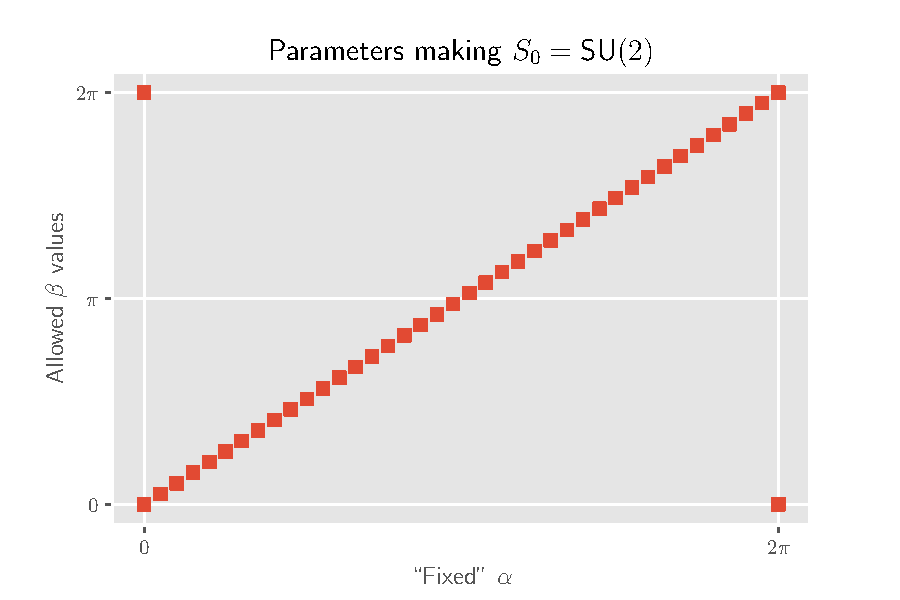
\includegraphics[width=\textwidth]{../su2/s0.pdf}
    \end{minipage}\hfill
    \begin{minipage}[c]{0.3\textwidth}
        \caption{Allowed parameters for $m = 1$}\label{fig:m=1}
    \end{minipage}
\end{figure}
\todo[linecolor=red,backgroundcolor=red!25,bordercolor=red]{figure titles are wrong /misleading}

\subsubsection{The $m = 2$ case}
In this case \cref{eq:solve} we have a free parameter $\theta$ to try and solve
\begin{equation}
    R_Y(\alpha)R_Z(\theta)R_Y(\alpha) = R_Y(\beta)
\end{equation}
which we can rewrite as
\begin{equation}
    R_Z(\theta) = R_Y(\beta - 2\alpha)
\end{equation}
which in general we cannot solve unless $\beta = 2\alpha$ where we can then take $\theta = 0$. We can again verify this (rather trivial) result numerically, doing a search for valid $\theta$ while varying $\alpha$ and $\beta$.
\begin{figure}[h]
    \begin{minipage}[c]{0.7\textwidth}
        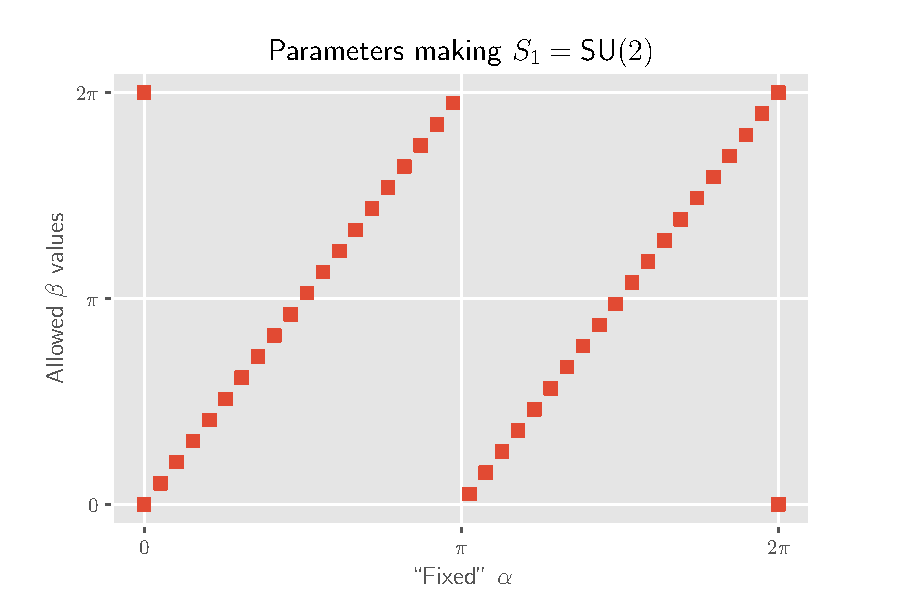
\includegraphics[width=\textwidth]{../su2/s1.pdf}
    \end{minipage}\hfill
    \begin{minipage}[c]{0.3\textwidth}
        \caption{Allowed parameters for $m = 2$}\label{fig:m=2}
    \end{minipage}
\end{figure}

Again we have $S_2\neq \SU{2}$, and it still fails quite badly.

\subsubsection{The $m = 3$ case}
The complexity is growing slowly where we now have two free parameters $\theta_1$ and $\theta_2$. Again moving the outer-most $Y$ rotations to the right hand side we have
\begin{align*}
    R_Y(\alpha)R_Z(\theta_1)R_Y(\alpha)R_Z(\theta_2)R_Y(\alpha) & = R_Y(\beta)            \\
    R_Z(\theta_1)R_Y(\alpha)R_Z(\theta_2)                       & = R_Y(\beta - 2\alpha).
\end{align*}
\begin{figure}[h]
    \begin{minipage}[c]{0.7\textwidth}
        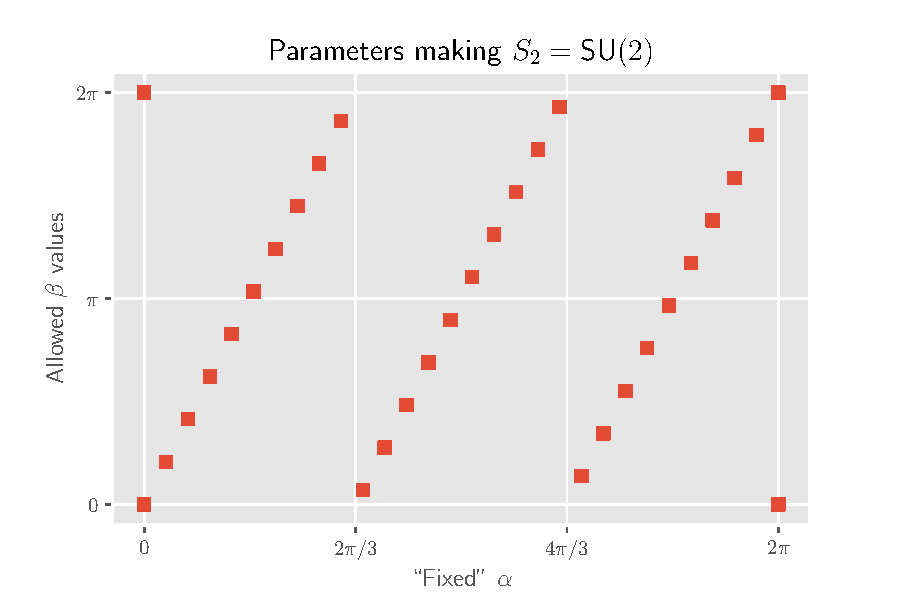
\includegraphics[width=\textwidth]{../su2/s2.pdf}
    \end{minipage}\hfill
    \begin{minipage}[c]{0.3\textwidth}
        \caption{Allowed parameters for $m = 3$}\label{fig:m=3}
    \end{minipage}
\end{figure}

\subsubsection{The $m = 4$ case}
Let's look at one more example before we say anything else. Unfortunately the number of points is lower than I'd like it to be, which is a result of not highly optimized code and impatience.
\begin{figure}[h]
    \begin{minipage}[c]{0.7\textwidth}
        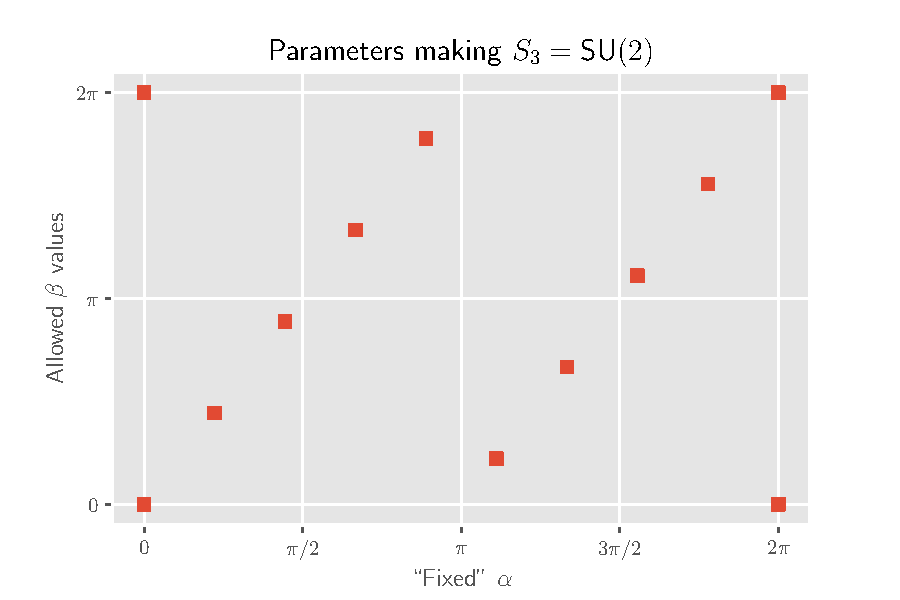
\includegraphics[width=\textwidth]{../su2/s3.pdf}
    \end{minipage}\hfill
    \begin{minipage}[c]{0.3\textwidth}
        \caption{Allowed parameters for $m = 4$}\label{fig:m=4}
    \end{minipage}
\end{figure}

The pattern I'm gleaning from these is that the allowed parameters all fall along the function
\begin{equation}
    h_m(x) = mx \mod 2\pi.
\end{equation}
By that I mean all the allowed pairs $(\alpha, \beta)\in[0, 2\pi]^2$ we've seen are all points in the graph of $h_m$.

\end{document}